\chapter{Antecedentes}
\label{capitulo4}
\lhead{Capítulo 4. \emph{Estado del Arte}}


El problema de evasión de obstáculos es un problema de planificación local de caminos. Entre las investigaciones que abordan este problema, existen dos variantes, las que dependen de la información global previa al momento de la planificación del camino y las investigaciones que dependen únicamente de la información de los sensores disponibles a bordo del vehículo al momento de la planificación del camino. En este capitulo se hace una revisión del estado del arte de ambas variantes mencionadas anteriormente, explorando la primera variante en la sección \ref{sec::prev-global}, la segunda variante en la sección \ref{sec::prev-local}, y profundizando en \textit{Learning high-speed flight in the wild} en la sección \ref{sec::prev-agile-autonomy}, que es el principal antecedente del desarrollo del presente trabajo.

\section{Investigaciones que dependen de la información global del entorno}
\label{sec::prev-global}

Este tipo de investigaciones separan sus algoritmos en dos etapas, una etapa fuera de linea (del inglés \textit{offline}) que se ejecuta antes de que el UAV comience el vuelo y una etapa en linea (del inglés \textit{online}) que se ejecuta durante la ejecución del vuelo. La etapa fuera de linea considera la información global del entorno, esto es, modelos del entorno, que pueden grafos, nube de puntos, entre otros; información del estado del entorno, que describen los eventos que ocurren en el entorno en el tiempo, como listas de vuelos consecutivos o posición de obstáculos programados en función del tiempo. La etapa en linea depende de los artefactos generados por la etapa fuera de linea y generalmente permiten que la complejidad de ejecución de la etapa en linea sea ligera. Sin embargo la dependencia de la etapa fuera de linea en la información global del entorno hace que este tipo de soluciones no sean viables en aplicaciones donde se desconoce a priori la información global del entorno. A continuación se describen brevemente algunas investigaciones que proponen este tipo de métodos.

En \cite{shi2018collision} se propone un método que genera en la etapa fuera de linea un camino libre de colisiones utilizando un algoritmo basado en A* que considera el grafo del espacio aéreo del entorno, una lista de sectores restringidos por situaciones climáticas o de regulaciones y la lista de los caminos en ejecución de otros UAV. Los caminos producidos por este algoritmo evitan obstáculos estáticos (en forma de sectores restringidos), así como también obstáculos dinámicos (en forma de caminos en ejecución). Este método tiene la ventaja de que si se mantiene correctamente la lista de caminos en ejecución, es posible orquestar la navegación de múltiples UAV en el entorno sin producir colisiones con obstáculos. Este tipo de métodos basados en A* tienen la desventaja de su etapa en linea no posee la capacidad de adaptarse a obstáculos no previstos en la etapa fuera de linea, en otras palabras, el camino se vuele completamente estático una vez que el UAV comienza el vuelo \cite{park2020boundary}; sin mencionar que su funcionamiento depende de que exista un grafo que modele el entorno correctamente.

Otros métodos tales como \cite{lifen2016path} utilizan campos potenciales artificiales para planificar caminos libres de colisión. La planificación de caminos por campos potenciales artificiales conciben al vehículo como una partícula inmersa en un campo de potencial cuyas variaciones locales reflejan la estructura del entorno \cite{bermudez2004aplicacion}, donde potenciales atractivos representan posiciones objetivo y potenciales repulsivos representan obstáculos, luego la trayectoria del vehículo es determinada iterativamente siguiendo el sentido de la fuerza producida por el potencial. En \cite{lifen2016path} se utiliza este concepto para producir caminos libres de colisión para la navegación de un UAV dentro de un entorno donde la ubicación de los obstáculos es conocida antes de comenzar el vuelo. La etapa fuera de linea en \cite{lifen2016path} calcula el camino a ejecutar siguiendo el potencial establecido por la información del entorno (obstáculos y posiciones objetivo) y la etapa en linea ejecuta este camino. Si bien \cite{lifen2016path} no lo hace, es posible que la etapa en linea recalcule localmente el camino inicial dado que se haya detectado algún obstáculo no previsto, sin embargo, esto introduce latencia en el sistema que pueden afectar la autonomía del vuelo. Este tipo de métodos basados en campos potenciales artificiales tienen la desventaja de que pueden hacer que el vehículo alcance mínimos locales de potencial que no permiten que el vehículo alcance su objetivo. Adicionalmente, estos métodos también son propensos a producir oscilaciones en la trayectoria, lo hace que la navegación no sea óptima y se desperdicie tiempo de vuelo, que justamente es uno de los recursos mas importantes para los UAV.


Por otro lado, en \cite{Zhang2019} se introduce P-CAL (Canales Alternativos Pre-calculados, del inglés \textit{Pre-computed Alternative Lanes}). Este método, en la etapa fuera de linea, dado un nube de puntos previamente calculada que codifica la información tridimensional del entorno, genera una colección de distintos caminos libres de colisión alternativos denominados canales (del inglés \textit{lanes}); entre cada canal adicionalmente se genera un camino de transición que permite cambiar de canal de forma fluida. Luego, en la etapa en linea, se alterna entre los distintos canales dependiendo de la presciencia de obstáculos no previstos. En otras palabras, P-CAL calcula un conjunto de caminos alternativos y luego alterna entre estos para evitar obstáculos imprevistos en el entorno. La detección de los obstáculos no previstos se hace comparando la información tridimensional predefinida del entorno con la lectura sensorial de un sensor LiDAR. La figura \ref{fig:P-CAL} muestra la nube de puntos del entorno previamente calculada, el resultado de la generación de los canales y caminos de transición; y el camino resultante de alternar canales para evadir obstáculos no previstos. El requerimiento de poseer una nube de puntos del entorno previo al vuelo del UAV, así como también la necesidad de utilizar un LiDAR para detectar obstáculos no previstos, hacen que este método no sea práctico para aplicaciones generales de evasión de obstáculos en donde no se tiene información previa del entorno o aquellas cuyos UAV no tengan la capacidad de utilizar un sensor LiDAR. 

\begin{figure}
    \centering
    \begin{subfigure}[b]{0.7\textwidth}
        \centering
        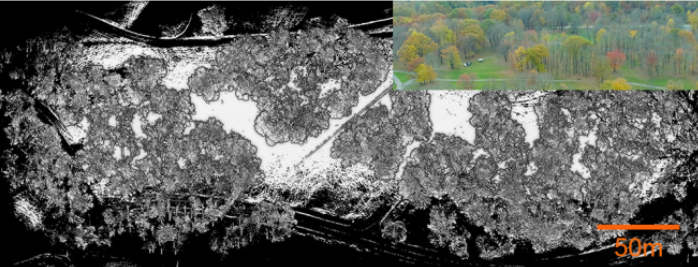
\includegraphics[width=\textwidth]{partes/img/P-CAL-map.png}
        \caption{Nube de puntos del entorno.}
    \end{subfigure}
    \hfill
    \begin{subfigure}[b]{0.7\textwidth}
        \centering
        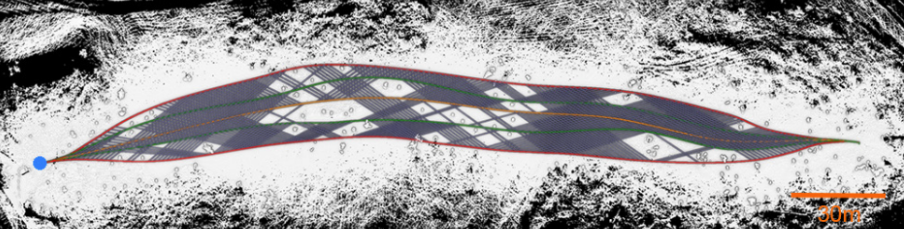
\includegraphics[width=\textwidth]{partes/img/P-CAL-lanes.png}
        \caption{Canales y caminos de transición.}
    \end{subfigure}
    \break
    \begin{subfigure}[b]{0.5\textwidth}
        \centering
        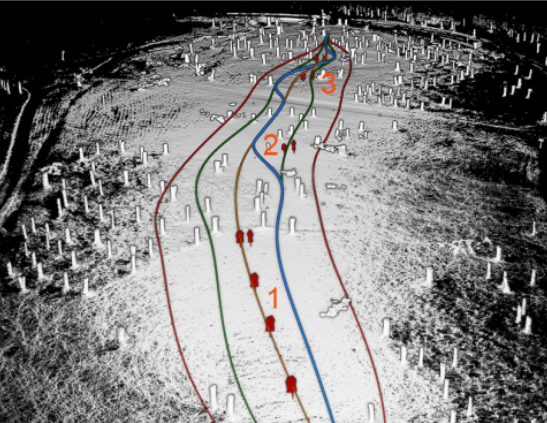
\includegraphics[width=\textwidth]{partes/img/P-CAL-results.png}
        \caption{Camino resultante.}
    \end{subfigure}
    \hfill
    
    \caption [P-CAL: Canales Alternativos Pre-calculados]{P-CAL, Canales Alternativos Pre-calculados \cite{Zhang2019}. \textbf{(a)} Nube de puntos del entorno previamente calculada. \textbf{(b)} Canales (amarillo, verde y rojo) y caminos de transición (azul) generados en la etapa fuera de linea. \textbf{(c)} Camino resultante (azul) de alternar entre canales para la evasión de los obstáculos no previstos 1, 2 y 3.}
    \label{fig:P-CAL}
\end{figure}

\section{Investigaciones que solo dependen de la información disponible a bordo del vehículo}

\label{sec::prev-local}

En la sección anterior exploramos algunas investigaciones que separan sus algoritmos en dos etapas: la etapa fuera de linea y la etapa en linea. En esta sección se van a explorar algunas investigaciones que se componen únicamente de una etapa que es análoga a la etapa en linea. Utilizando solamente la entrada sensorial de los sensores disponibles a bordo del UAV, estos métodos pueden evadir obstáculos no previstos en el entorno, así como navegar hacia su dirección objetivo. La interacción de estos métodos con el entorno es completamente reactiva y no se requiere de información previa para su funcionamiento.

En \cite{Yang2021} se utiliza una CNN probabilística para generar un mapa de profundidad acompañado de un mapa de confianza a partir de una imagen RBG del entorno. El mapa de confianza expresa que tan probable es que la información del mapa de profundidad sea correcta. Utilizando la información de ambos mapas, se calcula un mapa de profundidad efectiva tal como se expresa en la ecuación \ref{eq:P-CNN}, donde \jim{D} es el mapa de profundidad, \jim{C} es el mapa de confianza, \jim{v} es la velocidad del QUAV, \jim{a} es la aceleración del QUAV y \jim{T} es la longitud del intervalo de muestreo:

\begin{equation}
\label{eq:P-CNN}
    D_{eff}(i,j) = D(i,j) - (vT - \frac{aT^2}{2}) + \ln{(C(i,j))}
\end{equation}

Utilizando \jim{D_{eff}}, se calcula una mascara binaria de obstáculos \jim{D_{eff} > 0} que posteriormente se procesa agrupando los píxeles positivos (libres de obstáculos) en \textit{clusters}, cada \textit{cluster} representa una región libre de obstáculos. Una vez se tienen las regiones libres de obstáculos, se selecciona el centro de la región mas cercana como dirección de navegación. En la figura \ref{fig:P-CNN} se ilustra el mecanismo de evasión de obstáculos que se acaba de describir.

\begin{figure}[H]
    \centering
    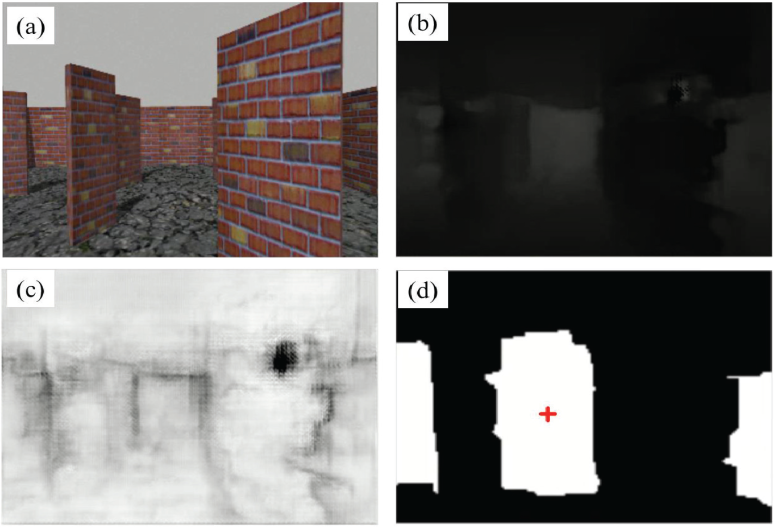
\includegraphics[scale=0.4]{partes/img/P-CNN.png}
    \caption[Mecanismo de evasión de obstáculos por CNN probabilística.]{Mecanismo\footnotemark de evasión de obstáculos por CNN probabilística \cite{Yang2021}. \textbf{(a)} Imagen RBG. \textbf{(b)} Mapa de profundidad. \textbf{(c)} Mapa de confianza. \textbf{(d)} Mascara de obstáculos y dirección de navegación seleccionada (cruz roja).} 
    \label{fig:P-CNN}
\end{figure}
\footnotetext{Obtenida de: \cite{Yang2021}}

El mecanismo de evasión de obstáculos por CNN probabilística propuesto en \cite{Yang2021} demostró ser efectivo para navegación arbitraria en interiores, sin embargo, como este método no considera el objetivo de la navegación, resulta poco útil para la mayoría de las aplicaciones.

Métodos que utilizan aprendizaje por reforzamiento abordan el problema de la evasión de obstáculos utilizando solamente la información disponible a bordo del QUAV. En \cite{Tu2023} se utiliza un algoritmo basado en \textit{Q-learning} para entrenar un agente dedicado a la evasión de obstáculos de un QUAV, donde la observación del estado del entorno viene dada por un mapa de profundidad y una imagen RBG; y donde el espacio de acciones es discreto, cada una representando una dirección de movimiento con respecto al campo de visión del QUAV. De forma similar, en \cite{Xue2021} se utiliza un algoritmo basado en el método Actor-Crítico suave (del inglés \textit{Soft Actor-Critic}), utilizando mapas de profundidad como observaciones del entorno pero utilizando un espacio de acciones continuas, donde una acción codifica un rango continuo de movimientos en las direcciones de los ejes \jim{y} y \jim{z} con respecto al marco de referencia del QUAV. 

El proceso de entrenamiento de estos métodos es considerablemente complicado, requiriendo múltiples redes neuronales para su funcionamiento. En la figura \ref{fig:prev-rl-training-process} se muestra el diagrama de flujo del proceso de entrenamiento utilizado en \cite{Xue2021}. Podemos observar inmediatamente la complejidad del proceso, requiriendo el entrenamiento simultaneo de siete CNNs. Otro inconveniente de estos métodos es la sensibilidad a la definición de la función de recompensa y las restricciones producidas por la representación del espacio de acciones.

\begin{figure}[H]
    \centering
    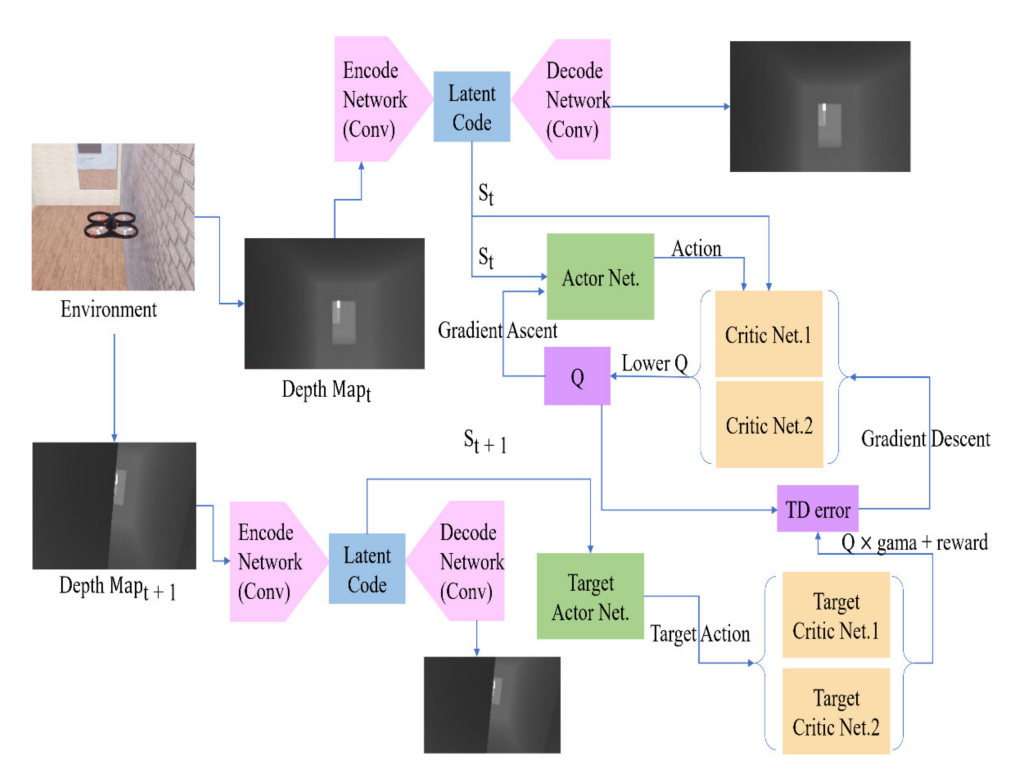
\includegraphics[scale=0.4]{partes/img/RL-training-process.png}
    \caption[Diagrama de flujo del proceso de entrenamiento utilizado en \textit{Vision Based Drone Obstacle Avoidance by Deep Reinforcement Learning}]{Diagrama de flujo del proceso de entrenamiento utilizado en \cite{Xue2021}.}
    \label{fig:prev-rl-training-process}
\end{figure}

Otro método que depende solamente de la información disponible a bordo del vehículo es \textit{Learning high-speed flight in the wild}, propuesto en \cite{Loquercio2021}, este método utiliza una variante del entrenamiento supervisado denominado entrenamiento por imitación (\textit{Imitation Learning} en inglés), en donde se genera una base de datos de entrenamiento utilizando un ``experto'' privilegiado dentro de un ambiente de simulación, para posteriormente aplicar entrenamiento supervisado sobre una política ``estudiante'' cuyo objetivo es aprender a generar trayectorias libres de colisión a partir de un mapa de profundidad del entorno y la mediciones inerciales del QUAV. En la siguiente sección, se profundiza en este método, que resulta ser el principal antecedente del desarrollo del presente trabajo.

\section{\textit{Learning high-speed flight in the wild}}

\label{sec::prev-agile-autonomy}

Tal como se menciono anteriormente, \textit{Learning high-speed flight in the wild} \cite{Loquercio2021} es un método que utiliza entrenamiento por imitación para entrenar una política de generación de trayectorias libres de colisión a partir de base de datos de ejemplos que son generados por un experto privilegiado dentro de un entorno de simulación. La figura \ref{fig:prev-agile-autonomy-overview} ilustra el funcionamiento de este método donde se aprecian sus tres componentes principales: El experto privilegiado, la política estudiante y la proyección de trayectorias. En las siguientes secciones se profundiza en el funcionamiento de cada uno de estos componentes.

\begin{figure}[H]
    \centering
    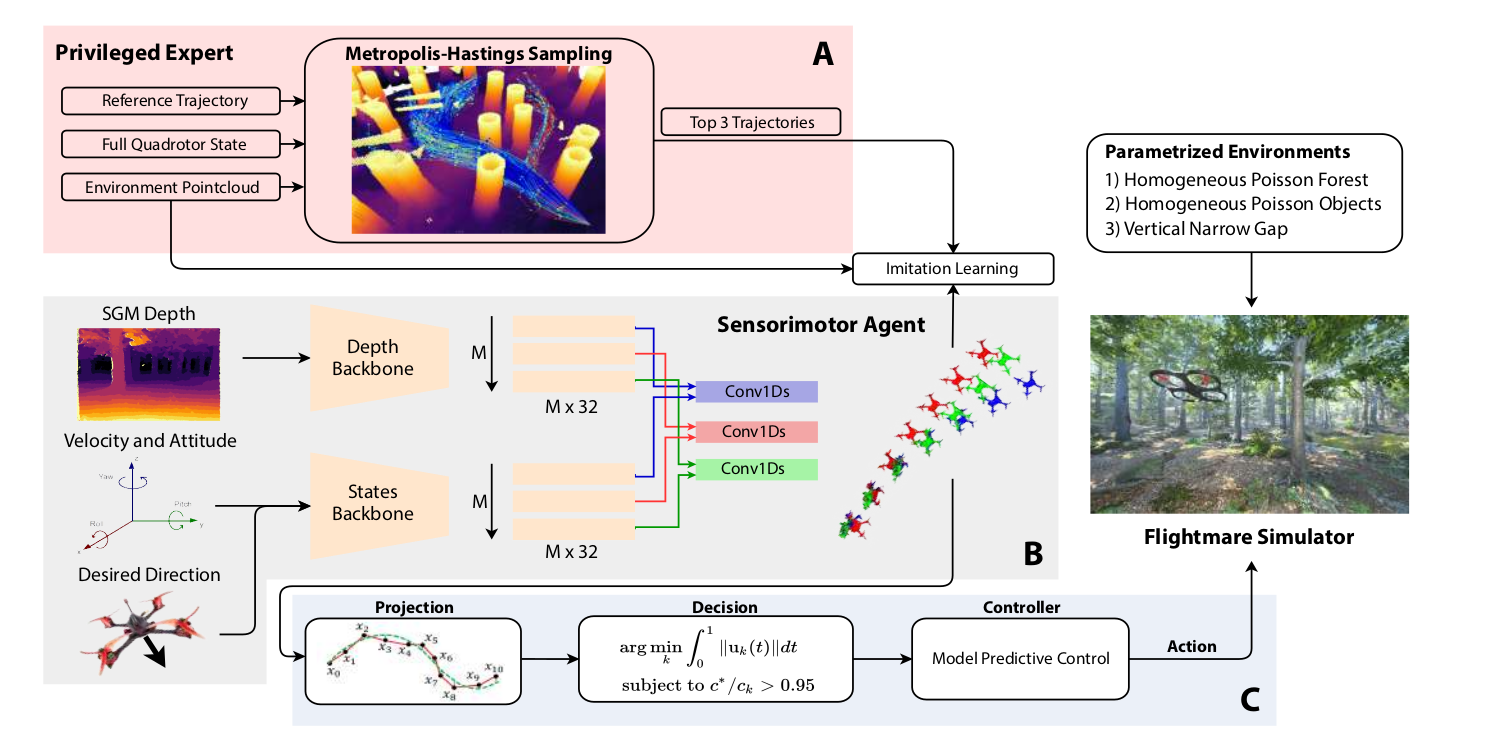
\includegraphics[scale=0.3]{partes/img/agile-autonomy-overview.png}
    \caption[Visión general del método propuesto en \textit{Learning high-speed flight in the wild}]{Visión general del método propuesto en \textit{Learning high-speed flight in the wild} \cite{Loquercio2021}. \textbf{(A)} El experto privilegiado genera una distribución de trayectorias libre de colisión que siguen una trayectoria de referencia. Las trayectorias generadas están condicionadas por la completa información de obstáculos del entorno. \textbf{(B)} La política estudiante es entrenada mediante entrenamiento supervisado para predecir las mejores tres trayectorias a partir un mapa de profundidad, mediciones inerciales del dron y una dirección objetivo. \textbf{(C)} Durante la ejecución, las predicciones de la política estudiante son proyectadas en el espacio de las trayectorias polinomiales y finalmente la trayectoria con el costo de predicción mas bajo es ejecutada por el modelo de control. }
    \label{fig:prev-agile-autonomy-overview}
\end{figure}

\subsection{El experto privilegiado} 

El experto privilegiado es un algoritmo de planificación de trayectorias basado en muestreo \cite{Loquercio2021}. El experto tiene conocimiento completo del estado del QUAV y de la configuración tridimensional del entorno (en forma de una nube de puntos tridimensional). El experto genera trayectorias libres de colisión \jim{\tau} que representan el estado deseado del QUAV \jim{x_{des} \in \mathbb{R}^{13}} durante el siguiente segundo, comenzando desde el estado inicial de QUAV, en otras palabras \jim{\tau(0) = x_0}. Para realizar esta tarea, se toman muestras de una distribución \jim{P} que codifica la distancia a los obstáculos y la proximidad a la trayectoria de referencia; esto es, la distribución \jim{P(\tau | \tau_{ref}, \mathcal{C})} es condicionada por la trayectoria de referencia \jim{\tau_{ref}} y la nube de puntos del entorno \jim{\mathcal{C} \in \mathbb{R}^{n \times 3}}. De acuerdo \jim{P}, la probabilidad de una trayectoria \jim{\tau} es alta si esta lejos de obstáculos en \jim{\mathcal{C}} y cerca de \jim{\tau_{ref}}. La ecuación \ref{eq:aoa-expert-P} muestra la definición de \jim{P} \cite{Loquercio2021}.

\begin{equation}
\label{eq:aoa-expert-P}
    P(\tau | \tau_{ref}, \mathcal{C}) = \frac{1}{Z} e^{-c(\tau, \tau_{ref}, \mathcal{C})}
\end{equation}

Donde \jim{Z = \int_{\tau} P(\tau | \tau_{ref}, \mathcal{C})} es el factor de normalización y \jim{c(\tau, \tau_{ref}, \mathcal{C}) \in \mathbb{R}^{+}} es una función de costo que indica la proximidad a la trayectoria de referencia y la distancia a los obstáculos. En la ecuación \ref{eq:aoa-expert-cost} define \jim{c} de acuerdo a \cite{Loquercio2021}.

\begin{equation}
\label{eq:aoa-expert-cost}
\begin{split}
    c(\tau, \tau_{ref}, \mathcal{C}) &  = \int_{0}^{1}{\lambda_{c} C_{collision}(\tau(t), \mathcal{C}) \, dt} \\
                                     & + \int_{0}^{1}{[\tau(t), - \tau_{ref}(t)]^{T} \, \mathcal{Q} \, [\tau(t) - \tau_{ref}(t)] \, dt}
\end{split}
\end{equation}

Donde \jim{\lambda_c = 1000}, \jim{\mathcal{Q}} es una matriz positiva que representa los pesos de los componentes del estado del vehículo, y \jim{C_{collision}} una función que cuantifica la distancia del QUAV a los puntos de \jim{\mathcal{C}}. Si \jim{r_q} es el radio del QUAV y \jim{d(z, \mathcal{C})} es la distancia de \jim{z \in \mathbb{R}^{3}} al punto mas cercano en \jim{\mathcal{C}}, la ecuación \ref{eq:aoa-expert-distance} define \jim{C_{collision}} de acuerdo a \cite{Loquercio2021}.

\begin{equation}
\label{eq:aoa-expert-distance}
    C_{collision}(\tau(t), \mathcal{C}) = \begin{cases}
        0                                               & \quad\text{\textbf{si} } d(\tau(t), \mathcal{C}) > 2 r_q \\
        4 - (\frac{d(\tau(t), \mathcal{C})}{r_q})^{2}   & \quad\text{\textbf{si} } d(\tau(t), \mathcal{C}) \leq 2 r_q
    \end{cases}
\end{equation}

Debido a que generalmente existe mas de una forma para evadir un obstáculo, la distribución es \jim{P} es multi-modal, haciendo que el calculo analítico de \jim{P} sea difícil de resolver. Para aproximar la densidad \jim{P}, el experto utiliza muestreo aleatorio mediante el algoritmo de \textit{Metropolis-hastings} \cite{hastings1970monte}. Para estimar \jim{P}, el algoritmo de \textit{Metropolis-hastings} necesita una función objetivo \jim{s(\tau) \propto  P(\tau | \tau_{ref}, \mathcal{C})}, en \cite{Loquercio2021} se utiliza \jim{s(\tau) = e^{-c(\tau, \tau_{ref}, \mathcal{C})}}. Luego, \cite{Loquercio2021} muestra que este algoritmo estima asintóticamente la distribución \jim{P}, por lo tanto, se asegura que las muestras de trayectorias cubren asintóticamente todas las modas de \jim{P}.

Para reducir la dimensionalidad del problema, el experto representa las trayectorias \jim{\tau} como curvas de Bezier con tres puntos de control (\jim{\tau \in \mathbb{R}^{3 \times 3}}) tal como se establece en \cite{mellinger2011minimum}, la longitud de estas trayectorias esta determinada por la rapidez promedio de ejecución deseada del QUAV. Adicionalmente, para reducir la complejidad de ejecución del experto, se discretizan las trayectorias en segmentos equitativamente espaciados de 0.1 segundos de duración y se evalúa la versión discreta de la ecuación \ref{eq:aoa-expert-cost}.

El experto luego se utiliza para generar una base de trayectorias libres de colisión mediante su ejecución en linea dentro de un ambiente de simulación. La figura \ref{fig:prev-aoa-expert-sample} se visualiza las muestras de \jim{P} generadas por el experto durante un paso de la simulación. Como trayectoria de referencia se utiliza una trayectoria global libre de obstáculos que se calcula utilizando el método de \cite{liu2018search} que comienza en una posición inicial y termina en la posición objetivo dentro del entorno. Se repite este proceso múltiples veces sobre distintos entornos de simulación. 

\begin{figure}[H]
    \centering
    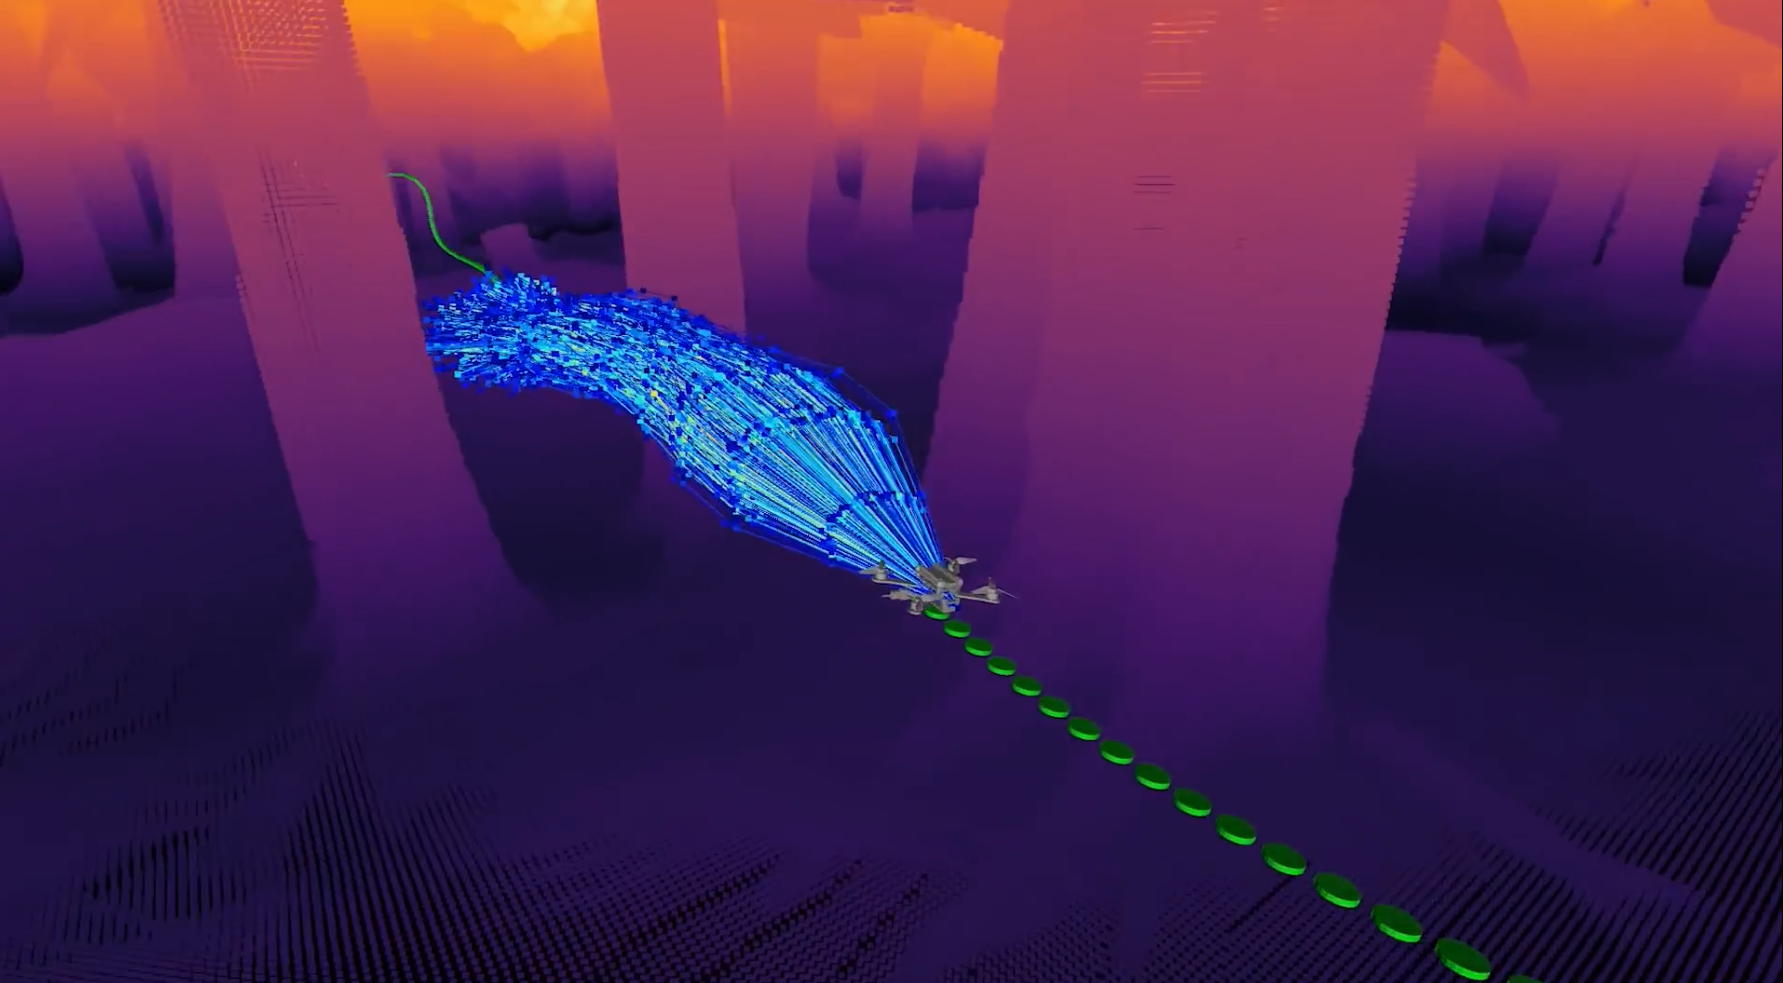
\includegraphics[scale=0.2]{partes/img/aoa-expert-sample.png}
    \caption[Visualización de las muestras de \jim{P} generadas por el experto durante un paso de la simulación.]{Visualización de las muestras de \jim{P} generadas por el experto durante un paso de la simulación. Los puntos verdes representan \jim{\tau_{ref}}.}
    \label{fig:prev-aoa-expert-sample}
\end{figure}


El conjunto de las mejores trayectorias generadas (mejores tres muestras por cada paso de la simulación) a lo largo de todas las ejecuciones se utiliza para formar una base de datos de trayectorias libres de colisión, cada ejemplo de la base de datos viene acompañado de un mapa de profundidad que se genera utilizando visión estereoscópica y del estado del QUAV (velocidad, rotación, posición y dirección objetivo). Si los entornos de simulación donde se realizan ejecuciones son los suficientemente variados (bosques, entornos urbanos, entornos de desastre, objetos aleatorios, entre otros) la base datos generada tiene la capacidad de utilizarse para entrenar políticas de evasión de obstáculos con un nivel de generalización aceptable \cite{Loquercio2021}. Es importante mencionar que debido a que la longitud de las muestras de \jim{P} están condicionadas por la rapidez promedio de ejecución deseada del QUAV, distintas velocidades de ejecución requieren diferentes base de datos, en otras palabras, para cada rapidez promedio de ejecución se necesita generar una base de datos distinta, y por lo tanto, las políticas de evasión de obstáculos entrenadas usando este método están condicionadas a la rapidez promedio del QUAV utilizada durante la generación de la base de datos.

\subsection{La política estudiante} 

\label{sec:aoa-student}

En contraste con el experto, la política estudiante (el estudiante) produce trayectorias libres de colisión en tiempo real utilizando solamente la información de los sensores disponible a bordo del QUAV. La información sensorial utilizada por el estudiante incluyen: un mapa de profundidad estimado utilizando visión estereoscópica, la velocidad y rotación del QUAV, y una dirección objetivo que es representada como un vector unitario que apunta hacia un punto de referencia un (1) segundo en el futuro con respecto al ultimo estado conocido del QUAV. Utilizando esta información y alguna base de datos generada por el experto privilegiado se puede entrenar un modelo que pueda cumplir con los requerimientos de la política estudiante.

En \cite{Loquercio2021} se modela la política estudiante como una red neuronal. La arquitectura de esta red contiene dos ramas que codifican distintas características: una rama convolucional, que codifica la información visual del entorno a partir de un mapa de profundidad \jim{D \in \mathbb{R}^{640 \times 480}}; y una rama que codifica el estado del QUAV a partir de la velocidad del vehículo \jim{v \in \mathbb{R}^{3}}, la rotación expresada como una matriz \jim{q \in \mathbb{R}^{9}}, y la dirección objetivo \jim{r \in \mathbb{R}^{3}} tal que \jim{\|r\| = 1}. 

La rama convolucional utiliza una instancia pre-entrenada de MobileNetV3 \cite{Howard2019} para extraer eficientemente las características visuales del mapa de profundidad. Estas características son posteriormente procesadas por una capa convolucional 1D para generar 3 vectores de tamaño 32, cada uno representando una moda de \jim{P}. 

La rama del estado del QUAV concatena \jim{v}, \jim{q} y \jim{r} y procesa el resultado mediante una red FC de 4 capas, cada una con \jim{[64,32,32,32]} numero de nodos y activaciones LeakyReLU; posteriormente el resultado es procesado por una capa convolucional 1D para generar 3 vectores de tamaño 32, una vez mas, cada uno representando una moda de \jim{P}.

Para cada moda, las codificaciones de la rama de estado y de la rama convolucional se concatenan y son procesadas por una red FC de 3 capas, cada una con \jim{[64,128,128]} numero de nodos y activaciones LeakyReLU. Finalmente, una ultima capa FC con activación LeakyReLU predice una trayectoria \jim{\tau} y costo de ejecución análogo al costo definido en la ecuación \ref{eq:aoa-expert-cost}. 


La salida de la red representa \jim{\mathbb{T}_n = \{ (\tau_{n}^{k}, c_k) | \, k \in [0,1,2] \}}, donde \jim{c_k \in \mathbb{R}^{+}} es el costo de ejecución de la trayectoria \jim{\tau_{n}^{k}} (análogo al definido en la ecuación \ref{eq:aoa-expert-cost}), nótese que cada \jim{k} representa una moda de \jim{P}. A diferencia del experto, las trayectorias predichas por el estudiante describen solamente el componente de la posición de la trayectoria, por esto, \jim{\tau_{n}^{k} \in \mathbb{R}^{10 \times 3}} y describe:

\begin{equation}
\label{eq:aoa-network-taun}
    \tau_{n}^{k} = {[p(t_i)]}_{i = 1}^{10}, \, t_i = \frac{i}{10}
\end{equation}

Donde \jim{p(t_i) \in \mathbb{R}^{3}} es la posición del QUAV en el tiempo \jim{t = t_i} relativo al estado actual \jim{x_0}.

La red neuronal se entrena utilizando entrenamiento supervisado por descenso de gradiente. La función de perdida para el entrenamiento tiene dos componentes, uno que representa el costo espacial entre la trayectoria predicha y la trayectoria generada por el experto; y otro que representa el costo de estimación de la función \jim{c} (definida en la ecuación \ref{eq:aoa-expert-cost}).

El componente espacial de la función de perdida es de tipo ``el ganador gana todo'' relajada R-WTA (del inglés \textit{Relaxed Winner-Takes-All)} definida como:

\begin{equation}
\label{eq:aoa-student-spacial-loss}
    \text{R-WTA}(\mathbb{T}_e, \mathbb{T}_n) = \sum_{i=0}^{|\mathbb{T}_e|} \sum_{k=0}^{|\mathbb{T}_n|} \alpha(\tau_{e,p}^{i}, \tau_{n}^{k}) {\|\tau_{e,p}^{i} - \tau_{n}^{k}\|}^2
\end{equation}

Donde \jim{\mathbb{T}_e} y \jim{\mathbb{T}_n} son el conjunto de trayectorias producidas por el experto y por el estudiante respectivamente, \jim{\tau_{e,p}} es el componente de la posición de \jim{\tau_e} y \jim{\alpha(.)} se define como:

\begin{equation}
\label{eq:aoa-student-spacial-alpha}
    \alpha(\tau_{e,p}^{i}, \tau_{n}^{k}) = \begin{cases}
        1 - \epsilon                            & \quad\text{\textbf{si} } {\|\tau_{e,p}^{i} - \tau_{n}^{k}\|}^2 \leq {\|\tau_{e,p}^{j} - \tau_{n}^{k}\|}^2 \, \forall i \ne j \\
        \frac{\epsilon}{|\mathbb{T}_n| - 1}     & \quad\text{\textbf{en caso contrario}}
    \end{cases}
\end{equation}

Con \jim{\epsilon = 0.05}. Esta definición hace que intuitivamente se asocie una trayectoria \jim{\tau_{e}^{i} \in \mathbb{T}_e} con la trayectoria mas cercana predicha por el estudiante \jim{\tau_{n}^{k} \in \mathbb{T}_n}, asignándole un peso de \jim{1 - \epsilon = 0.95}; dejando un peso de \jim{\epsilon / (|\mathbb{T}_n| - 1) = 0.025} para el resto de las predicciones, de ahí el nombre ``el ganador gana todo''. Esta formulación permite que la red pueda aprender el comportamiento multi-modal de las trayectorias generadas por el experto.

El componente de estimación de la función \jim{c} esta dado por la suma de diferencias cuadradas entre el valor a estimar y la predicción de la red. El valor a estimar se obtiene para cada predicción utilizando la asociación generada por el componente R-WTA, digamos que \jim{h(k)} retorna el índice de la trayectoria del experto asociada con la predicción numero \jim{k}. Finalmente, la función de perdida utilizada para el entrenamiento de la red neuronal que modela al estudiante es \cite{Loquercio2021}:

\begin{equation}
\label{eq:aoa-student-spacial-loss-full}
    L(\mathbb{T}_e, \mathbb{T}_n) = 10 \cdot \text{R-WTA}(\mathbb{T}_e, \mathbb{T}_n) + \frac{1}{10} \cdot \sum_{k=0}^{|\mathbb{T}_e|} [c_k - c(\tau_{n}^{k}, \tau_{e,p}^{h(k)}, \mathcal{C})]^2
\end{equation}

Esta función de perdida es promediada sobre un \textit{batch} de 8 muestras y se minimiza utilizando descenso de gradiente con una tasa de aprendizaje de \jim{1 \times 10^{-3}} \cite{Loquercio2021}.

\subsection{Proyección de trayectorias} 

\label{sec:prev-aoa-traj}

Las trayectorias predichas por la política estudiante son proyectadas al espacio de los polinomios de grado \jim{N} con \jim{N \geq 3} para cada eje independientemente. Esta representación polinómica asegura continuidad en posición, velocidad, aceleración y facilita la viabilidad dinámica de la trayectoria \cite{mellinger2011minimum}. Por ejemplo, para el eje x, se define la proyección polinómica \jim{\mu_x(t) = a_x^T \cdot T(t)}, donde \jim{a_x^T = [a_0, a_1, ..., a_N]} y \jim{T(t) = [1, t, ..., t^{N -1}, t^{N}]}. El termino de proyección \jim{a_x} se obtiene resolviendo el siguiente problema de optimización:

\begin{equation}
\label{eq:aoa-traj-proj}
\begin{split}
    \min_{a_x} \sum_{i=1}^{10} & (\tau_{n,x}^{k,i} - a_x^T \cdot T(\frac{i}{10}))^{2} \\
    \text{\textbf{sujeto a:}} & \\
                     & p_x(0) - a_x^T \cdot T(0) = 0 \\
                     & v_x(0) - a_x^T \cdot \frac{dT}{dt}(0) = 0 \\
                     & a_x(0) - a_x^T \cdot \frac{d^2 T}{{dt}^2}(0) = 0 \\
\end{split}
\end{equation}

Donde \jim{\tau_{n,x}^{k,i}} es el componente en el eje x del elemento numero \jim{i} de \jim{\tau_{n}^{k}}, y \jim{p_x(0), v_x(0), a_x(0)} son el componente x de la posición, velocidad y aceleración del QUAV obtenidas del ultimo estado \jim{x_0}. Adicionalmente, para evitar cambios abruptos en la velocidad durante el vuelo, se limita la rapidez promedio del polinomio a un valor definido \jim{v_{des}} que coincide con la rapidez promedio de ejecución de la base de datos con la que se entrenó la política estudiante. Para ello, se escala el tiempo \jim{t} del polinomio \jim{\mu(t)} por un factor \jim{\beta = v_{des} / v_\mu} donde \jim{v_\mu = \| \mu(0) - \mu(1) \|}.

Una vez que todas las trayectorias han sido proyectadas, se escoge una para ejecutarse. Para esto, se seleccionan las trayectorias que cumplan con \jim{c^{*} / c_k \geq 0.95 \, (c^{*} = \min_k c_k)} y se selecciona aquella de que tenga el menor valor de entrada acuerdo al criterio establecido por \cite{mellinger2011minimum}. Esto refuerza continuidad temporal de las trayectorias. Por ejemplo, si se esta esquivando un obstáculo por la derecha no es ideal navegar hacia la izquierda en la siguiente iteración, a no ser que sea estrictamente necesario por la apariencia del obstáculo. Finalmente, se obtienen valores de posición, velocidad y aceleración de la trayectoria seleccionada y se envían al FCU para su ejecución.

\section{Resumen}

Este capítulo abordó el problema de la evasión de obstáculos, centrándose en dos variantes de planificación local de caminos: aquellas que requerían información global previa y las que se basaban únicamente en la información de los sensores a bordo del vehículo. La sección \ref{sec::prev-global} exploró investigaciones relacionadas con la primera variante, mientras que la sección \ref{sec::prev-local} se centró en la segunda. Además, se profundizó en \textit{Learning high-speed flight in the wild} en la sección \ref{sec::prev-agile-autonomy}, destacando su papel como un antecedente crucial para el desarrollo del presente trabajo. Este capítulo proporcionó una visión del estado actual en el campo, resaltando las perspectivas relevantes para la resolución del problema de evasión de obstáculos para QUAVs.

En el siguiente capítulo se describirá la implementación de la solución propuesta por este trabajo, teniendo en cuenta el contexto de la plataforma disponible, así como también fundamentando la selección del algoritmo de evasión de obstáculos y detallando sus componentes de implementación.
    
   